\newsec{Dimensione interatomica}

Usando sempre la legge di Bragg (\ref{eq:bragg}), invertendola:
\begin{equation}
2d = \frac{n\lambda}{\sin \theta}
\end{equation}
vogliamo ricavare i passi reticolari dei cristalli di \ce{LiF} e \ce{KCl}.
Nello specifico lavoriamo sempre ad un regime di $ V_\text{EHT} = 30 \unit{kV} $, $ i = 40 \unit{\micro A} $ e $ V_\text{alimentazione} = 506 \unit{V} $, e fissiamo sul cammino ottico il filtro di nichel: studiamo solo la riga di emissione $ K_{\alpha} $.

Dopo aver localizzato la posizione approssimativa dell'unico picco di emissione (al prim'ordine, quindi $ n=1 $) ben identificabile con il contatore Geiger, passiamo direttamente alle scansioni fini dello spettro (passo $ 1/6 \unit{\degree} $) in quell'intorno.
Come prima: interpoliamo sui massimi, e consideriamo come errore la somma in quadratura della HWHM del picco, e dell'errore sul posizionamento della scala.

\begin{table}
\centering \small
\begin{tabular}{cccc|cccc}
$2\theta_{\ce{LiF}}$ & $\delta 2\theta_{\ce{LiF}}$ & $\nu_{\ce{LiF}}$ & $\delta \nu_{\ce{LiF}}$ & $2\theta_{\ce{KCl}}$ & $\delta 2\theta_{\ce{KCl}}$ & $\nu_{\ce{KCl}}$ & $\delta \nu_{\ce{KCl}}$ \\
\hline
42.00 & 0.08 & 16.1 & 0.9 & 25.17 & 0.08 & 11.75 & 0.17\\
42.17 & 0.08 & 18.1 & 1.0 & 25.33 & 0.08 & 10.10 & 0.16\\
42.33 & 0.08 & 22.1 & 1.1 & 25.50 & 0.08 & 8.75 & 0.15\\
42.50 & 0.08 & 29.1 & 1.2 & 25.67 & 0.08 & 9.45 & 0.15\\
42.67 & 0.08 & 46.2 & 1.5 & 25.83 & 0.08 & 10.80 & 0.16\\
42.83 & 0.08 & 78 & 2 & 26.00 & 0.08 & 12.25 & 0.18\\
43.00 & 0.08 & 219 & 3 & 26.17 & 0.08 & 13.30 & 0.18\\
43.17 & 0.08 & 386 & 4 & 26.33 & 0.08 & 19.8 & 0.2\\
43.33 & 0.08 & 506 & 5 & 26.50 & 0.08 & 43.3 & 0.3\\
43.50 & 0.08 & 564 & 5 & 26.67 & 0.08 & 131.1 & 0.6\\
43.67 & 0.08 & 589 & 5 & 26.83 & 0.08 & 294.0 & 0.9\\
43.83 & 0.08 & 636 & 6 & 27.00 & 0.08 & 562.2 & 1.2\\
44.00 & 0.08 & 594 & 5 & 27.17 & 0.08 & 696.1 & 1.3\\
44.17 & 0.08 & 432 & 5 & 27.33 & 0.08 & 817.8 & 1.4\\
44.33 & 0.08 & 266 & 4 & 27.50 & 0.08 & 829.6 & 1.4\\
44.50 & 0.08 & 139 & 3 & 27.67 & 0.08 & 794.3 & 1.4\\
44.67 & 0.08 & 36.6 & 1.4 & 27.83 & 0.08 & 573.2 & 1.2\\
44.83 & 0.08 & 18.1 & 1.0 & 28.00 & 0.08 & 307.6 & 0.9\\
45.00 & 0.08 & 15.9 & 0.9 & 28.17 & 0.08 & 153.8 & 0.6\\
45.17 & 0.08 & 17.2 & 0.9 & 28.33 & 0.08 & 68.3 & 0.4\\
45.33 & 0.08 & 15.1 & 0.9 & 28.50 & 0.08 & 36.9 & 0.3\\
45.50 & 0.08 & 14.6 & 0.9 & 28.67 & 0.08 & 23.2 & 0.2\\
  -   &  -   &   -   &  -   & 28.83 & 0.08 & 22.0 & 0.2\\
  -   &  -   &   -   &  -   & 29.00 & 0.08 & 20.4 & 0.2\\
  -   &  -   &   -   &  -   & 29.17 & 0.08 & 19.5 & 0.2
\end{tabular}
\caption{Dati relativi ai grafici nelle figure (\ref{fig:LiF}) e (\ref{fig:KCl}), cioè alla scansioni fini degli spettri di \ce{LiF} (a sinistra) e di $ \ce{KCl} $ (a destra): gli angoli sono indicati in $ \unit{\degree} $ in scala $ 2\theta $, mentre le frequenze in conteggi al $ \unit{s} $ (su un intervallo di tempo di $ \Delta t = 20 \unit{s} $).}
\label{tab:LiFKCl}
\end{table}


\subsection{Cristallo di \ce{LiF}}

In \cref{tab:LiFKCl} e in \cref{fig:LiF} sono raccolti i dati relativi alle frequenze dei conteggi in $ \Delta t = 20 \unit{s} $ per angoli $ 2\theta \in [42, 45.5] \unit{\degree} $.

\begin{figure}
\centering
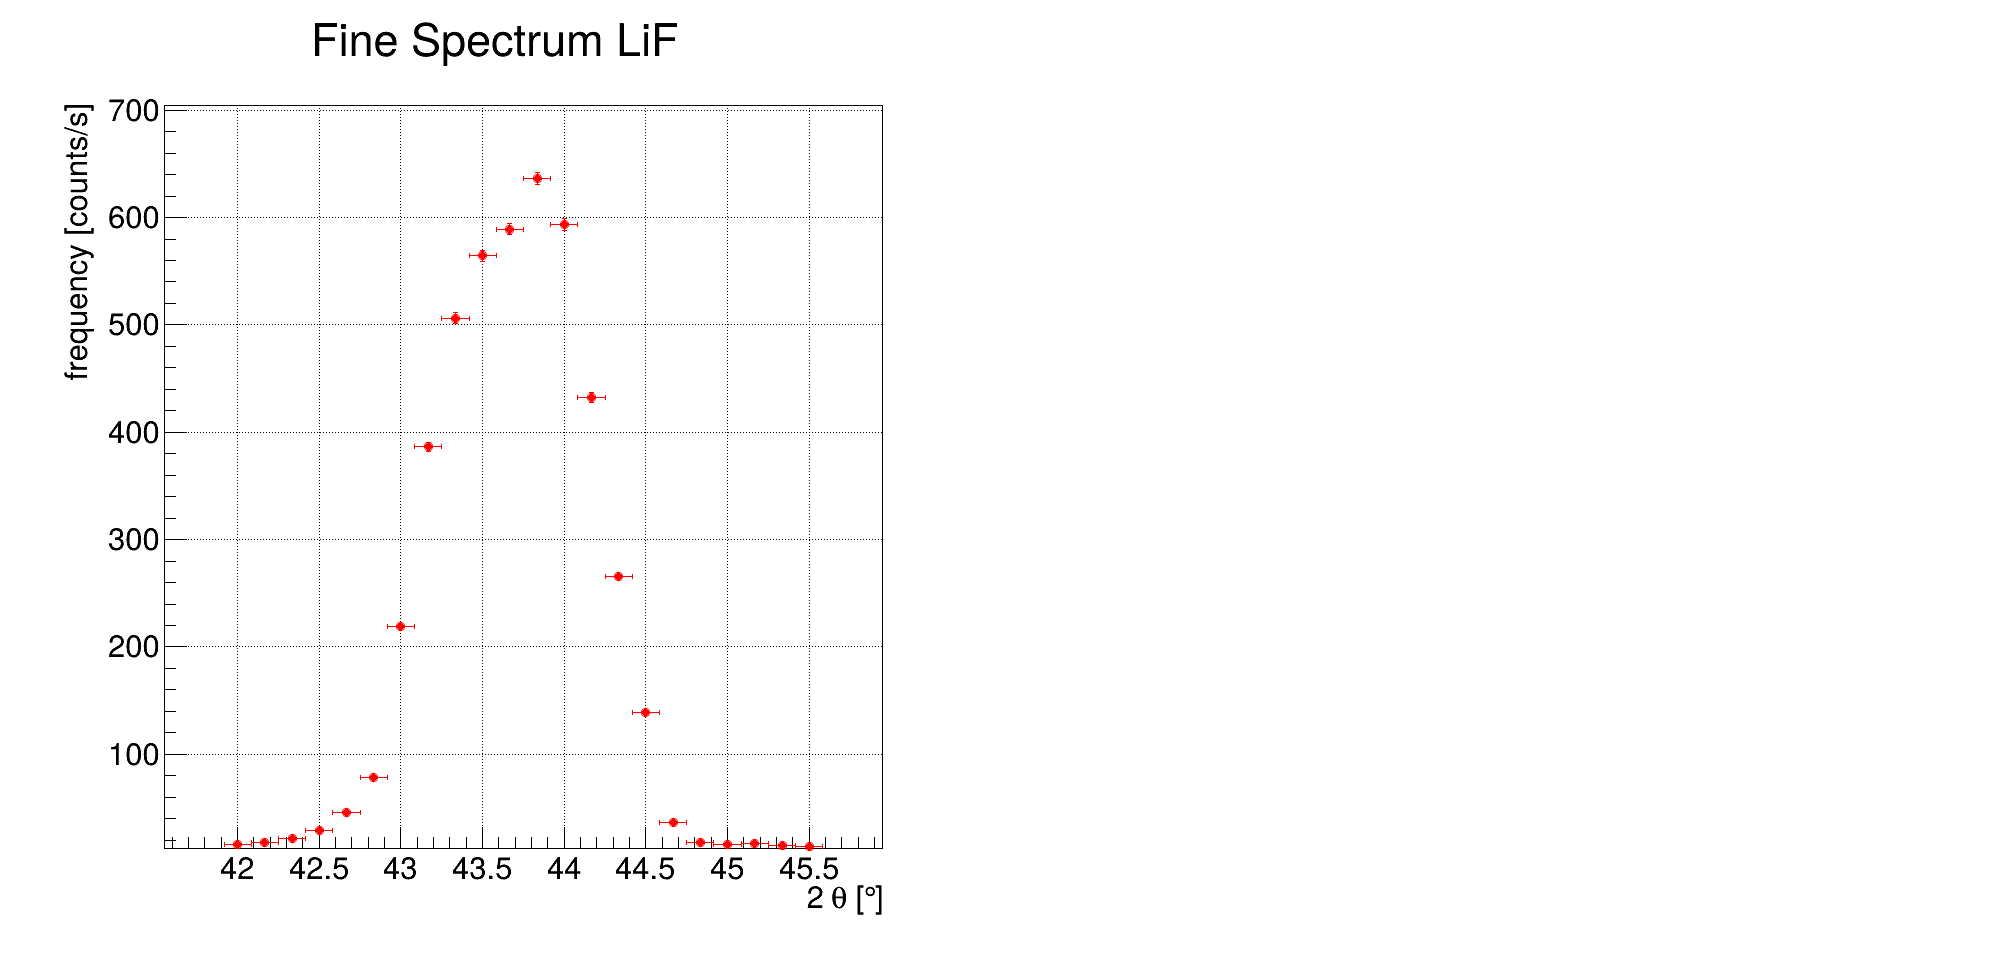
\includegraphics[width=0.85\textwidth]{./figs/LiF.png}
\caption{Frequenze di rilevazione dei raggi X in $ \Delta t = 20 \unit{s} $ al variare dell'angolo (misurato in gradi sulla scala $ 2 \theta $) di diffrazione del fascio sul cristallo di \ce{LiF}.}
\label{fig:LiF}
\end{figure}



Da questi otteniamo la stima:
\begin{equation}
\theta_{2,\ce{LiF}} = (21.9 \pm 0.4) \unit{\degree} \xrightarrow[]{\text{Bragg}} 2d_{\ce{LiF}} = (4.14 \pm 0.07) \unit{\angstrom}
\end{equation}
che è compatibile con il valore nominale $ 2d_{\ce{LiF}}^\text{theo} = (4.035 \pm 0.001) \unit{\angstrom}$ (con $Z = 1.59$, accettato al $5 \%$).

Correggendo per il bias sistematico di $ (0.7 \pm 0.4) \unit{\degree} $ otteniamo una stima corretta:
\begin{equation}
\theta_{2,\ce{LiF}}' = (22.6 \pm 0.6) \unit{\degree} \xrightarrow[]{\text{Bragg}} 2d_{\ce{LiF}}' = (4.02 \pm 0.09) \unit{\angstrom}
\end{equation}
che diventa compatibile con il valore tabulato con $ Z = 0.897 $ (accettabile al $ 5\% $).

\subsection{Cristallo di \ce{KCl}}

In \cref{tab:LiFKCl} e in \cref{fig:KCl} sono raccolti i dati relativi alle frequenze dei conteggi in $ \Delta t = 20 \unit{s} $ per angoli $ 2\theta \in [25, 29] \unit{\degree} $.

\begin{figure}
\centering
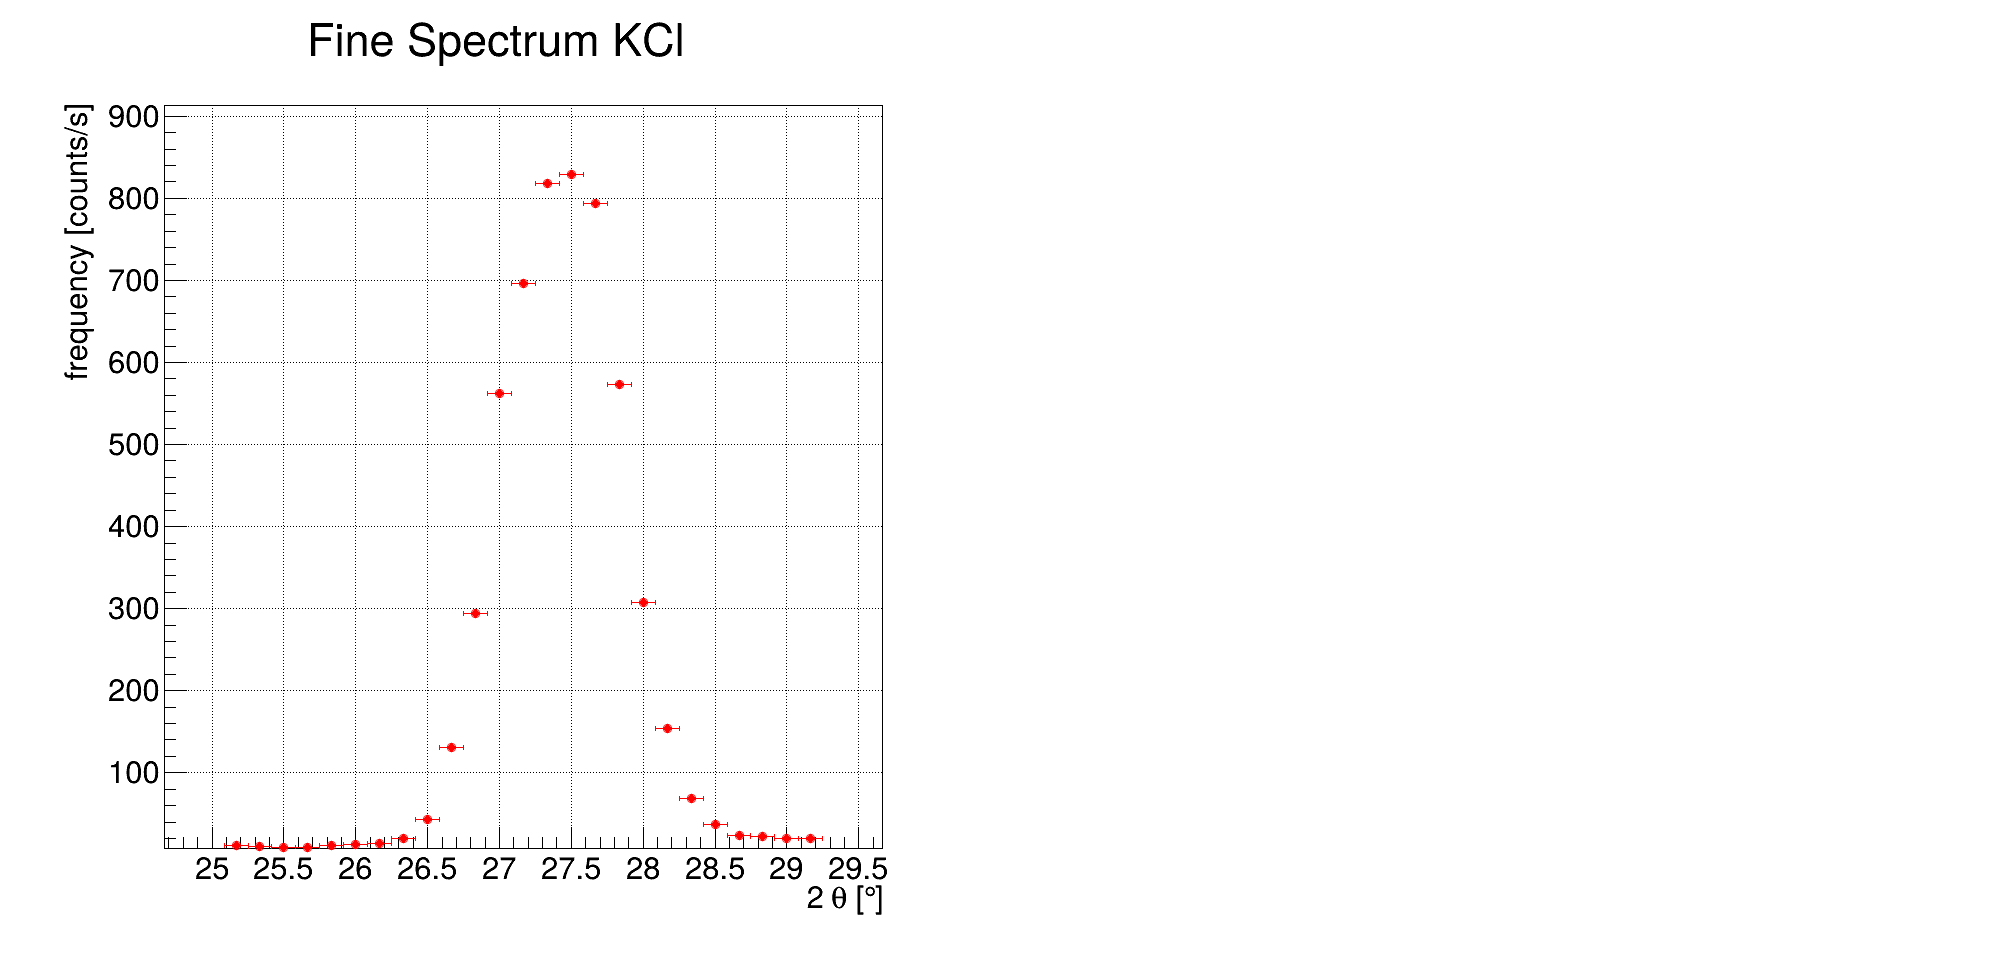
\includegraphics[width=0.85\textwidth]{./figs/KCl.png}
\caption{Frequenze di rilevazione dei raggi X in $ \Delta t = 20 \unit{s} $ al variare dell'angolo (misurato in gradi sulla scala $ 2 \theta $) di diffrazione del fascio sul cristallo di \ce{KCl}.}
\label{fig:KCl}
\end{figure}

Da questi otteniamo la stima:
\begin{equation}
\theta_{2,\ce{KCl}} = (13.7 \pm 0.4) \unit{\degree} \xrightarrow[]{\text{Bragg}} 2d_{\ce{KCl}} = (6.5 \pm 0.2) \unit{\angstrom}
\end{equation}
che è compatibile con il valore nominale $ 2d_{\ce{KCl}}^\text{theo} = (6.29 \pm 0.01) \unit{\angstrom}$ (con $Z = 1.12$, accettato al $5 \%$).

Correggendo per il bias sistematico di $ (0.7 \pm 0.4) \unit{\degree} $ otteniamo una stima corretta:
\begin{equation}
\theta_{2,\ce{KCl}}' = (14.4 \pm 0.6) \unit{\degree} \xrightarrow[]{\text{Bragg}} 2d_{\ce{KCl}}' = (6.2 \pm 0.2) \unit{\angstrom}
\end{equation}
che diventa compatibile con il valore tabulato con $ Z = 0.345 $ (accettabile al $ 5 \% $).

